% Define center type column
\newcolumntype{Y}{>{\centering\arraybackslash}X}
\newcolumntype{P}[1]{>{\centering\arraybackslash}m{#1}}
\newcolumntype{T}[1]{>{\small\centering\arraybackslash}m{#1}}
\renewcommand\tabularxcolumn[1]{m{#1}}

%spacing
\renewcommand{\arraystretch}{2.5}
\begin{table}
    \small
    \begin{tabularx}{\textwidth}{T{3cm}  P{5cm}  Y}
        Matching & Pattern & Text with occurrences underlined \\
        \hline
        \textbf{Regular expression} \cite{RM-704} & $P=$ GAT$(\mathrm{TA}\mid \mathrm{O})(\mathrm{CAT})^*$ & ~\underline{GATTA}AT\underline{GATOCATCAT}A \\
        %Error bound~\cite{landau1986efficient} (for ED~\cite{levenshtein1966binary}) & $P=$ GATTACAT &  AT\underline{GATTAACAT}ATA, $\mathrm{ED}(P,T[2..10])=1$ \\
        Don't care \cite{fischer1974string} & \begin{minipage}{3cm}\centering $P=$ GAT??CAT \\ \footnotesize{The ? match any other characters.}\end{minipage} & \underline{GATTACAT}A\underline{GATOACAT}AC\\
        %
        \textbf{Gapped consecutive} \cite{bille2022gapped} & \begin{minipage}{5cm}\centering $P_1=$ GATTA $P_2=$ TAC  $a=2$, $b=6$\\ \footnotesize{Consecutive occurrences $(i,j)$ of $(P_1,P_2)$ and s.t. $j-i \in [a,b]$ } \end{minipage} &  AGG\underline{GATTAC}TAC, distance between $P_1$ and $P_2$ $6-3=3 \in [a,b]$\\
        %
        Degenerate \cite{abrahamson1987generalized}  & \begin{minipage}{5cm}\centering $P=$ GATTACAT \\ \footnotesize{Some positions can match several characters.}\end{minipage} &   {\renewcommand{\arraystretch}{1} A$\left\{
            \begin{array}{l}
                \mathrm{T}  \\
                \mathrm{C}
            \end{array}\right\}$\underline{GAT}$\left\{
            \begin{array}{l}
                \mathrm{\underline{T}}  \\
                \mathrm{A}
            \end{array}\right\} \mathrm{\underline{ACAT}A}$} \\
        %
        Generalized degenerate \cite{alzamel_et_al:LIPIcs:2018:9323}  & \begin{minipage}{5cm}\centering $P=$ GATTACAT \\ \footnotesize{Some positions match a set  strings of a fixed length.} \end{minipage} &   {\renewcommand{\arraystretch}{1} AT$\left\{
            \begin{array}{l}
                \mathrm{\underline{G}}  \\
                \mathrm{T}
            \end{array}\right\}
        \mathrm{\underline{AT}}\left\{
            \begin{array}{l}
                \mathrm{\underline{TA}}  \\
                \mathrm{AT}
            \end{array}\right\} \mathrm{\underline{CAT}A}$} \\
        %
        %
        Elastic degenerate \cite{iliopoulos2021efficient}  & \begin{minipage}{5cm}\centering $P=$ GATTACAT \\ \footnotesize{Some positions match a set of strings (length can vary).} \end{minipage} &   {\renewcommand{\arraystretch}{1} AT\underline{GAT}$\left\{
            \begin{array}{l}
                \mathrm{\underline{TA}}  \\
                \mathrm{A}
            \end{array}\right\} \mathrm{\underline{CAT}A}$} \\
        %
        Abelian/Jumbled \cite{eres2004permutation} & \begin{minipage}{5cm}\centering $P=$ GATTACAT \\ \footnotesize{Characters can be in reordered.} \end{minipage} &  AGAG\underline{TATGATCA}GT\\
        %
        Weighted \cite{thompson1994clustal} & \begin{minipage}{5cm}\centering \footnotesize{Each position is given a character probability distribution.}\\ GATTA has a cumulative probability $>0.07$.\end{minipage} & 
        \begin{minipage}{4.5cm} \footnotesize
            \renewcommand{\arraystretch}{1}
            \begin{tabular}{c|ccccc}
                 & 0    & 1 & 2 & 3 & 4 \\
                \hline
                A & 0    & \underline{1} & 0.25 & 0 & \underline{0.75}\\
                C & 0.25 & 0 & 0.25 & 0 & 0.25\\
                G & \underline{0.75} & 0  & 0.25 & 0.5 & 0\\
                T & 0    & 0  & \underline{0.25} & \underline{0.5} & 0\\
            \end{tabular}
        \end{minipage} \\
        %
        Order preserving \cite{kim2014order,kubica2013linear}  & $P =$ 1 5 3 4 6 2 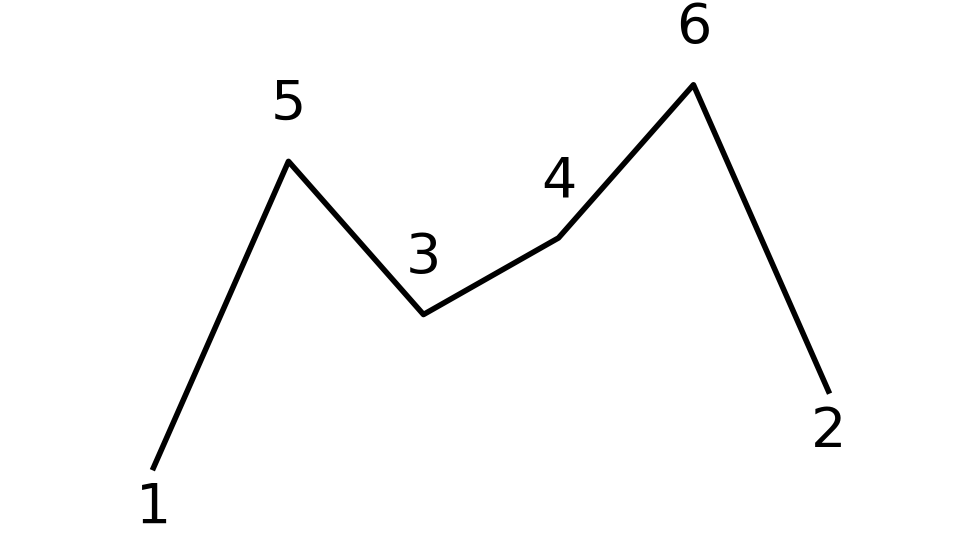
\includegraphics[width=3.5cm]{Introduction/op_P.png} \footnotesize{Characters must have the same relative order.} &  \underline{2 7 4 5 8 3} \underline{1 20 15 16 25 6}  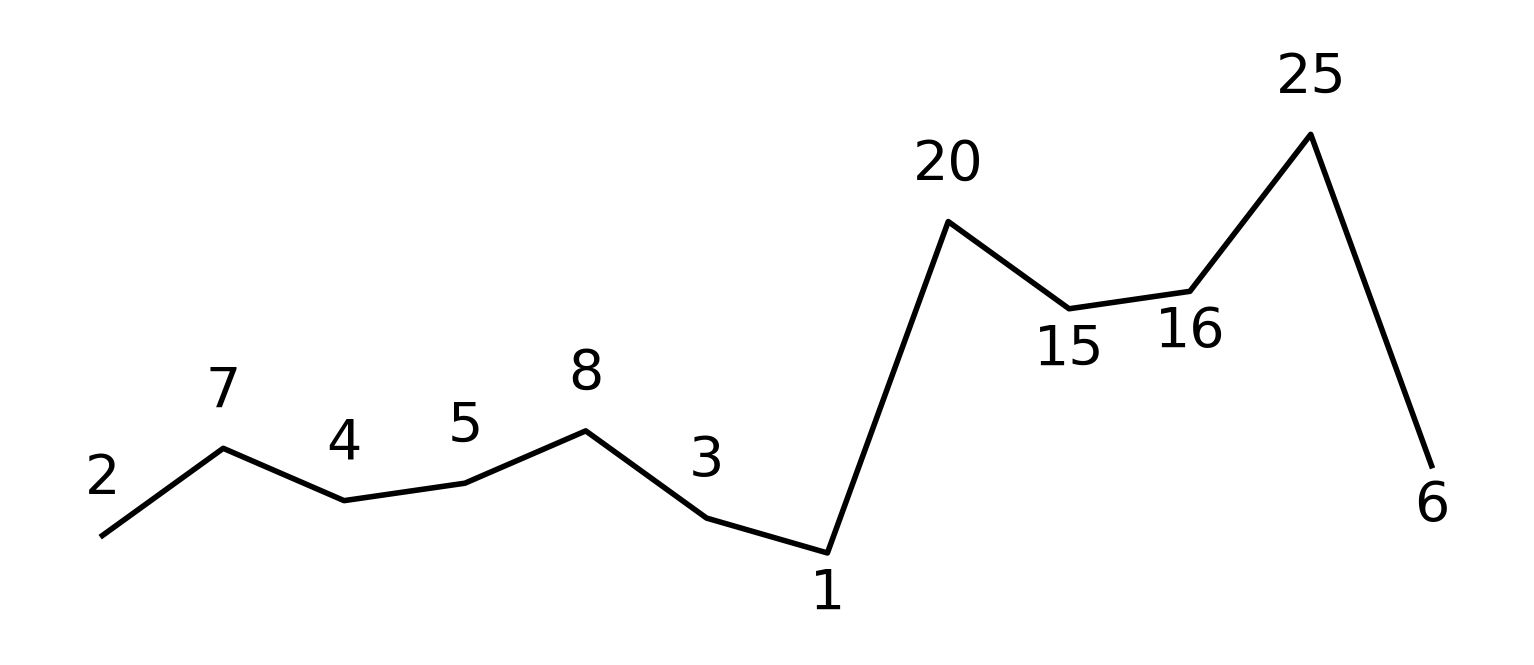
\includegraphics[width=6cm]{Introduction/op_T.png} \\
        %
        Parametrized \cite{baker1993theory} & \begin{minipage}{5cm} \centering $P=$ GATTACAT\\ \footnotesize{Characters can be renamed with a bijection} \end{minipage} &  \begin{minipage}{4cm}\centering OPO\underline{POGGODOG}O \\ \small{A:O, C:D, G:P, T:G} \end{minipage} \\
    \end{tabularx}
    \caption{Example for various matching models, in bold those we study in this thesis.}
    \label{fig:intro:match_model}
\end{table}


\renewcommand{\arraystretch}{1}